\chapter{Análisis visual}
\labch{vis-anal}
\begin{figure}[h!]
	\centering
	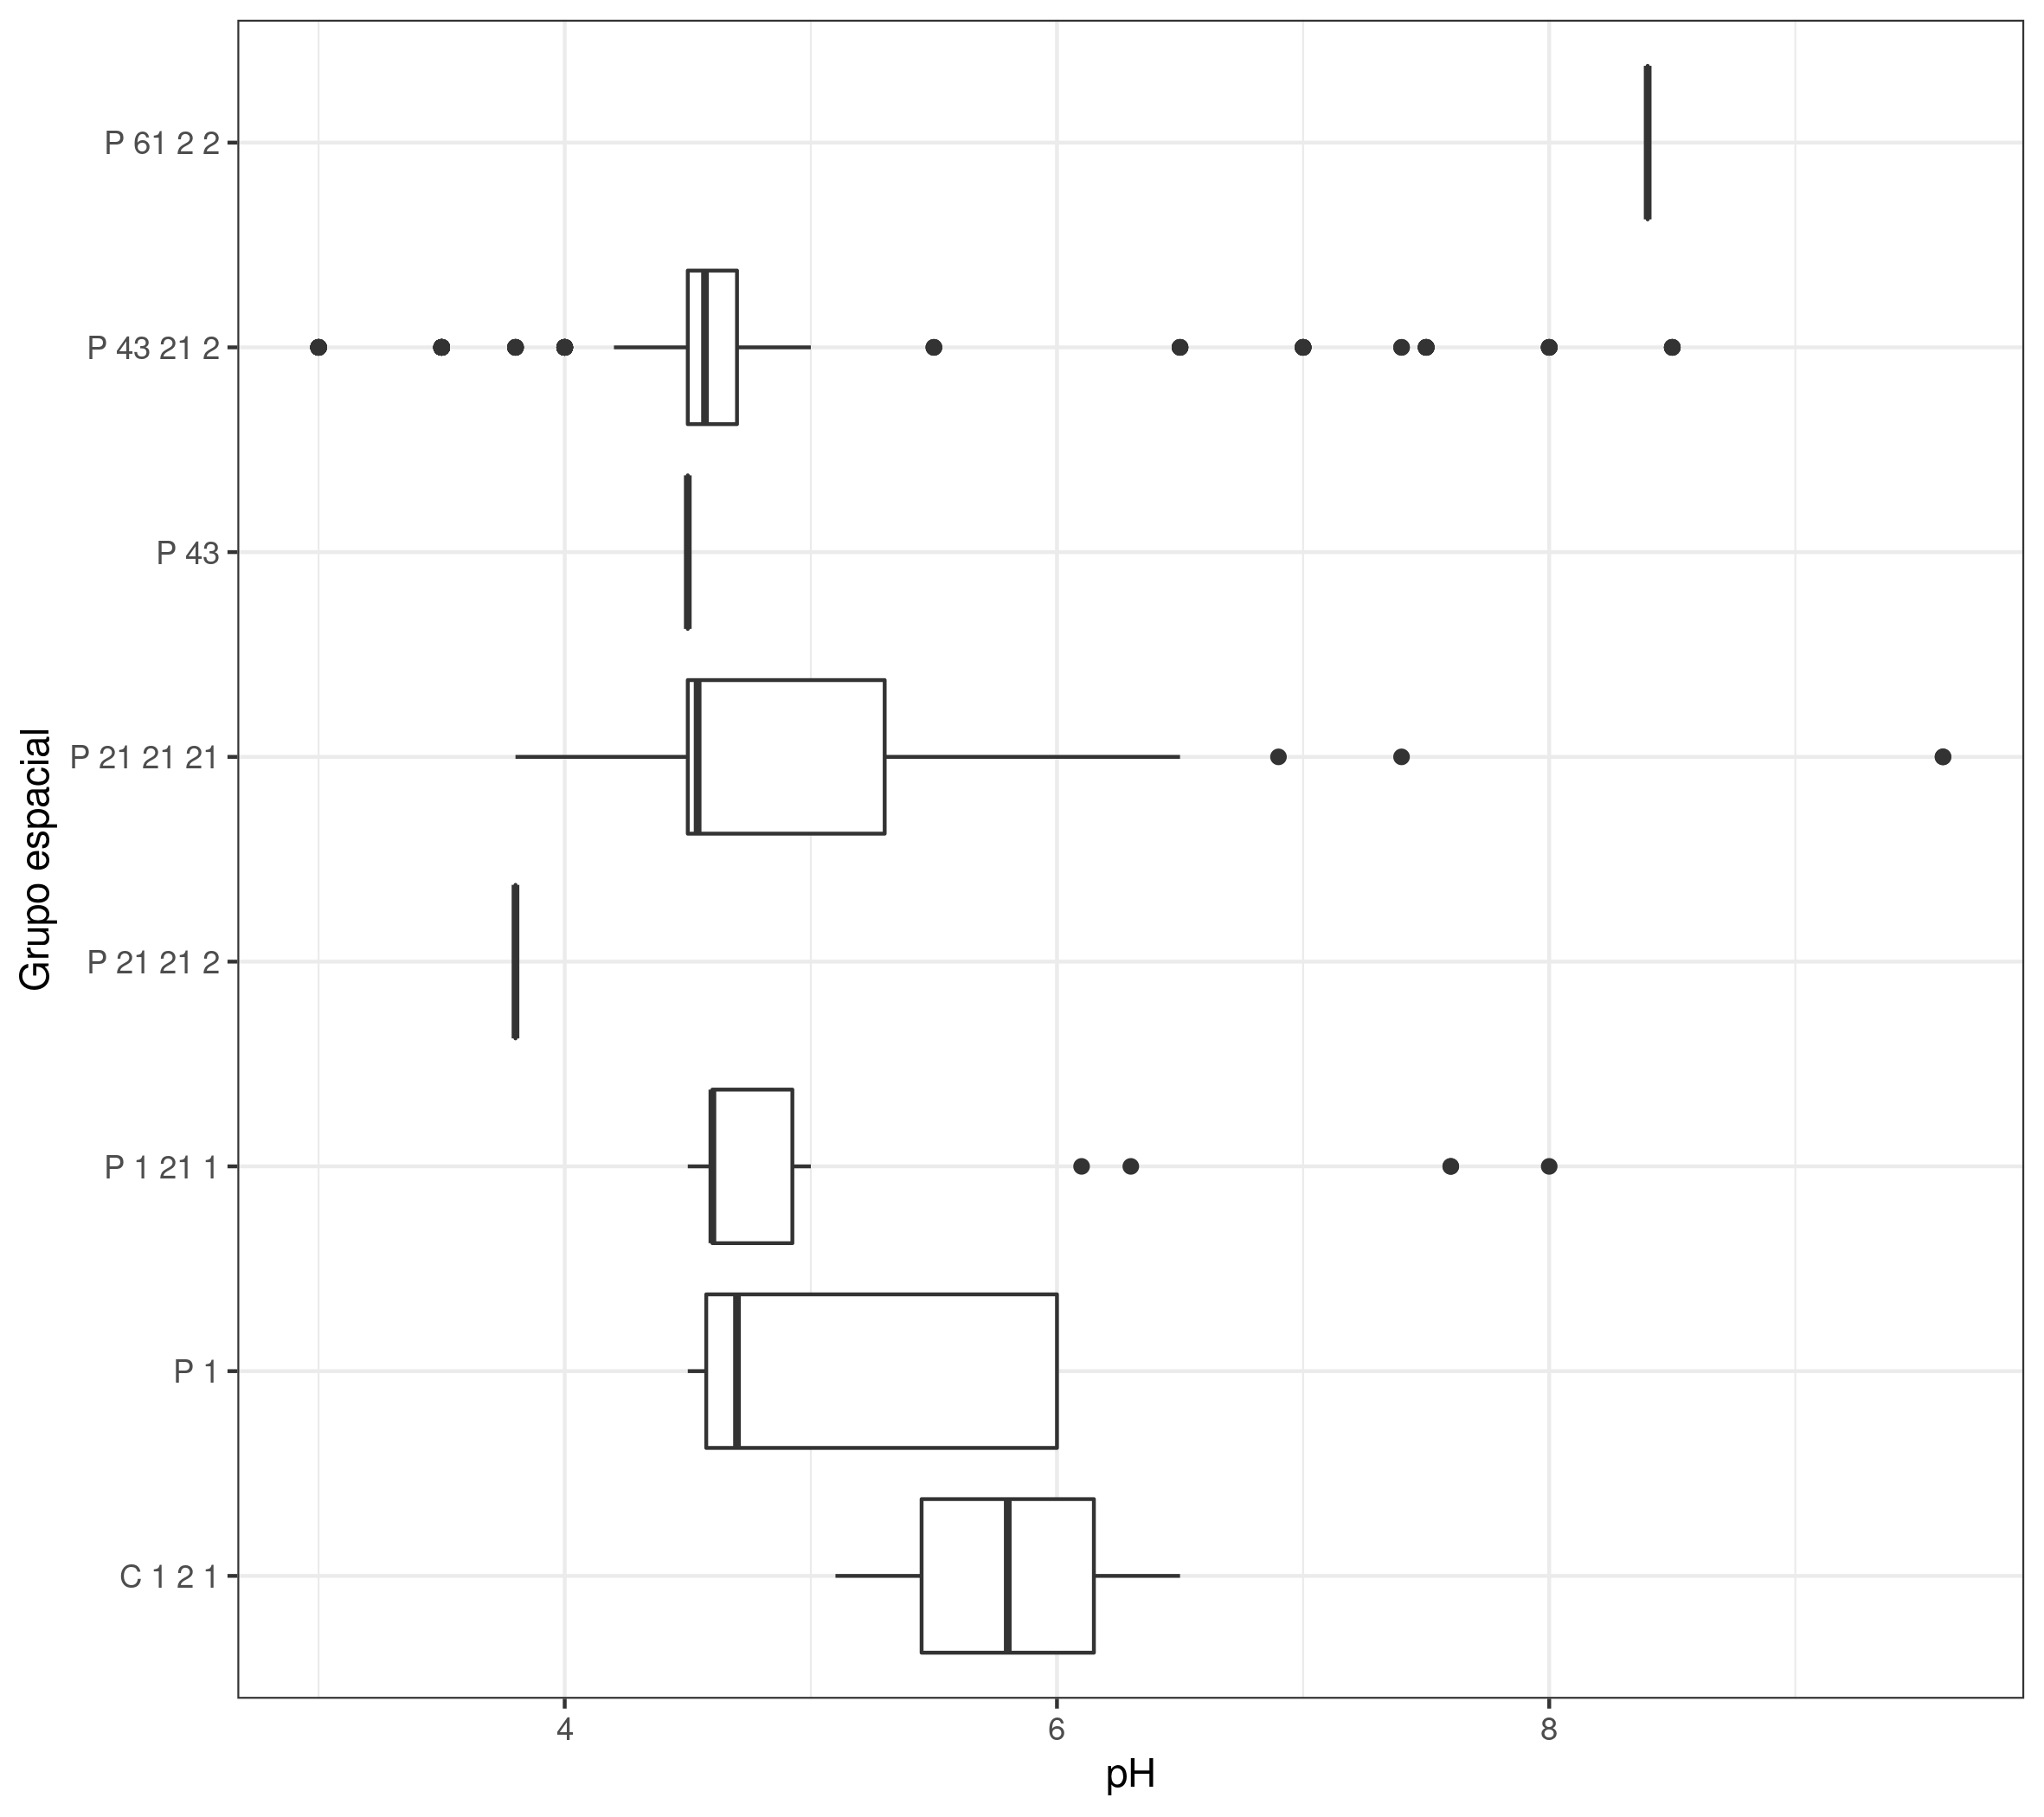
\includegraphics[width=0.8\textwidth]{imgs/box_pH_by_gpo_P00698}
	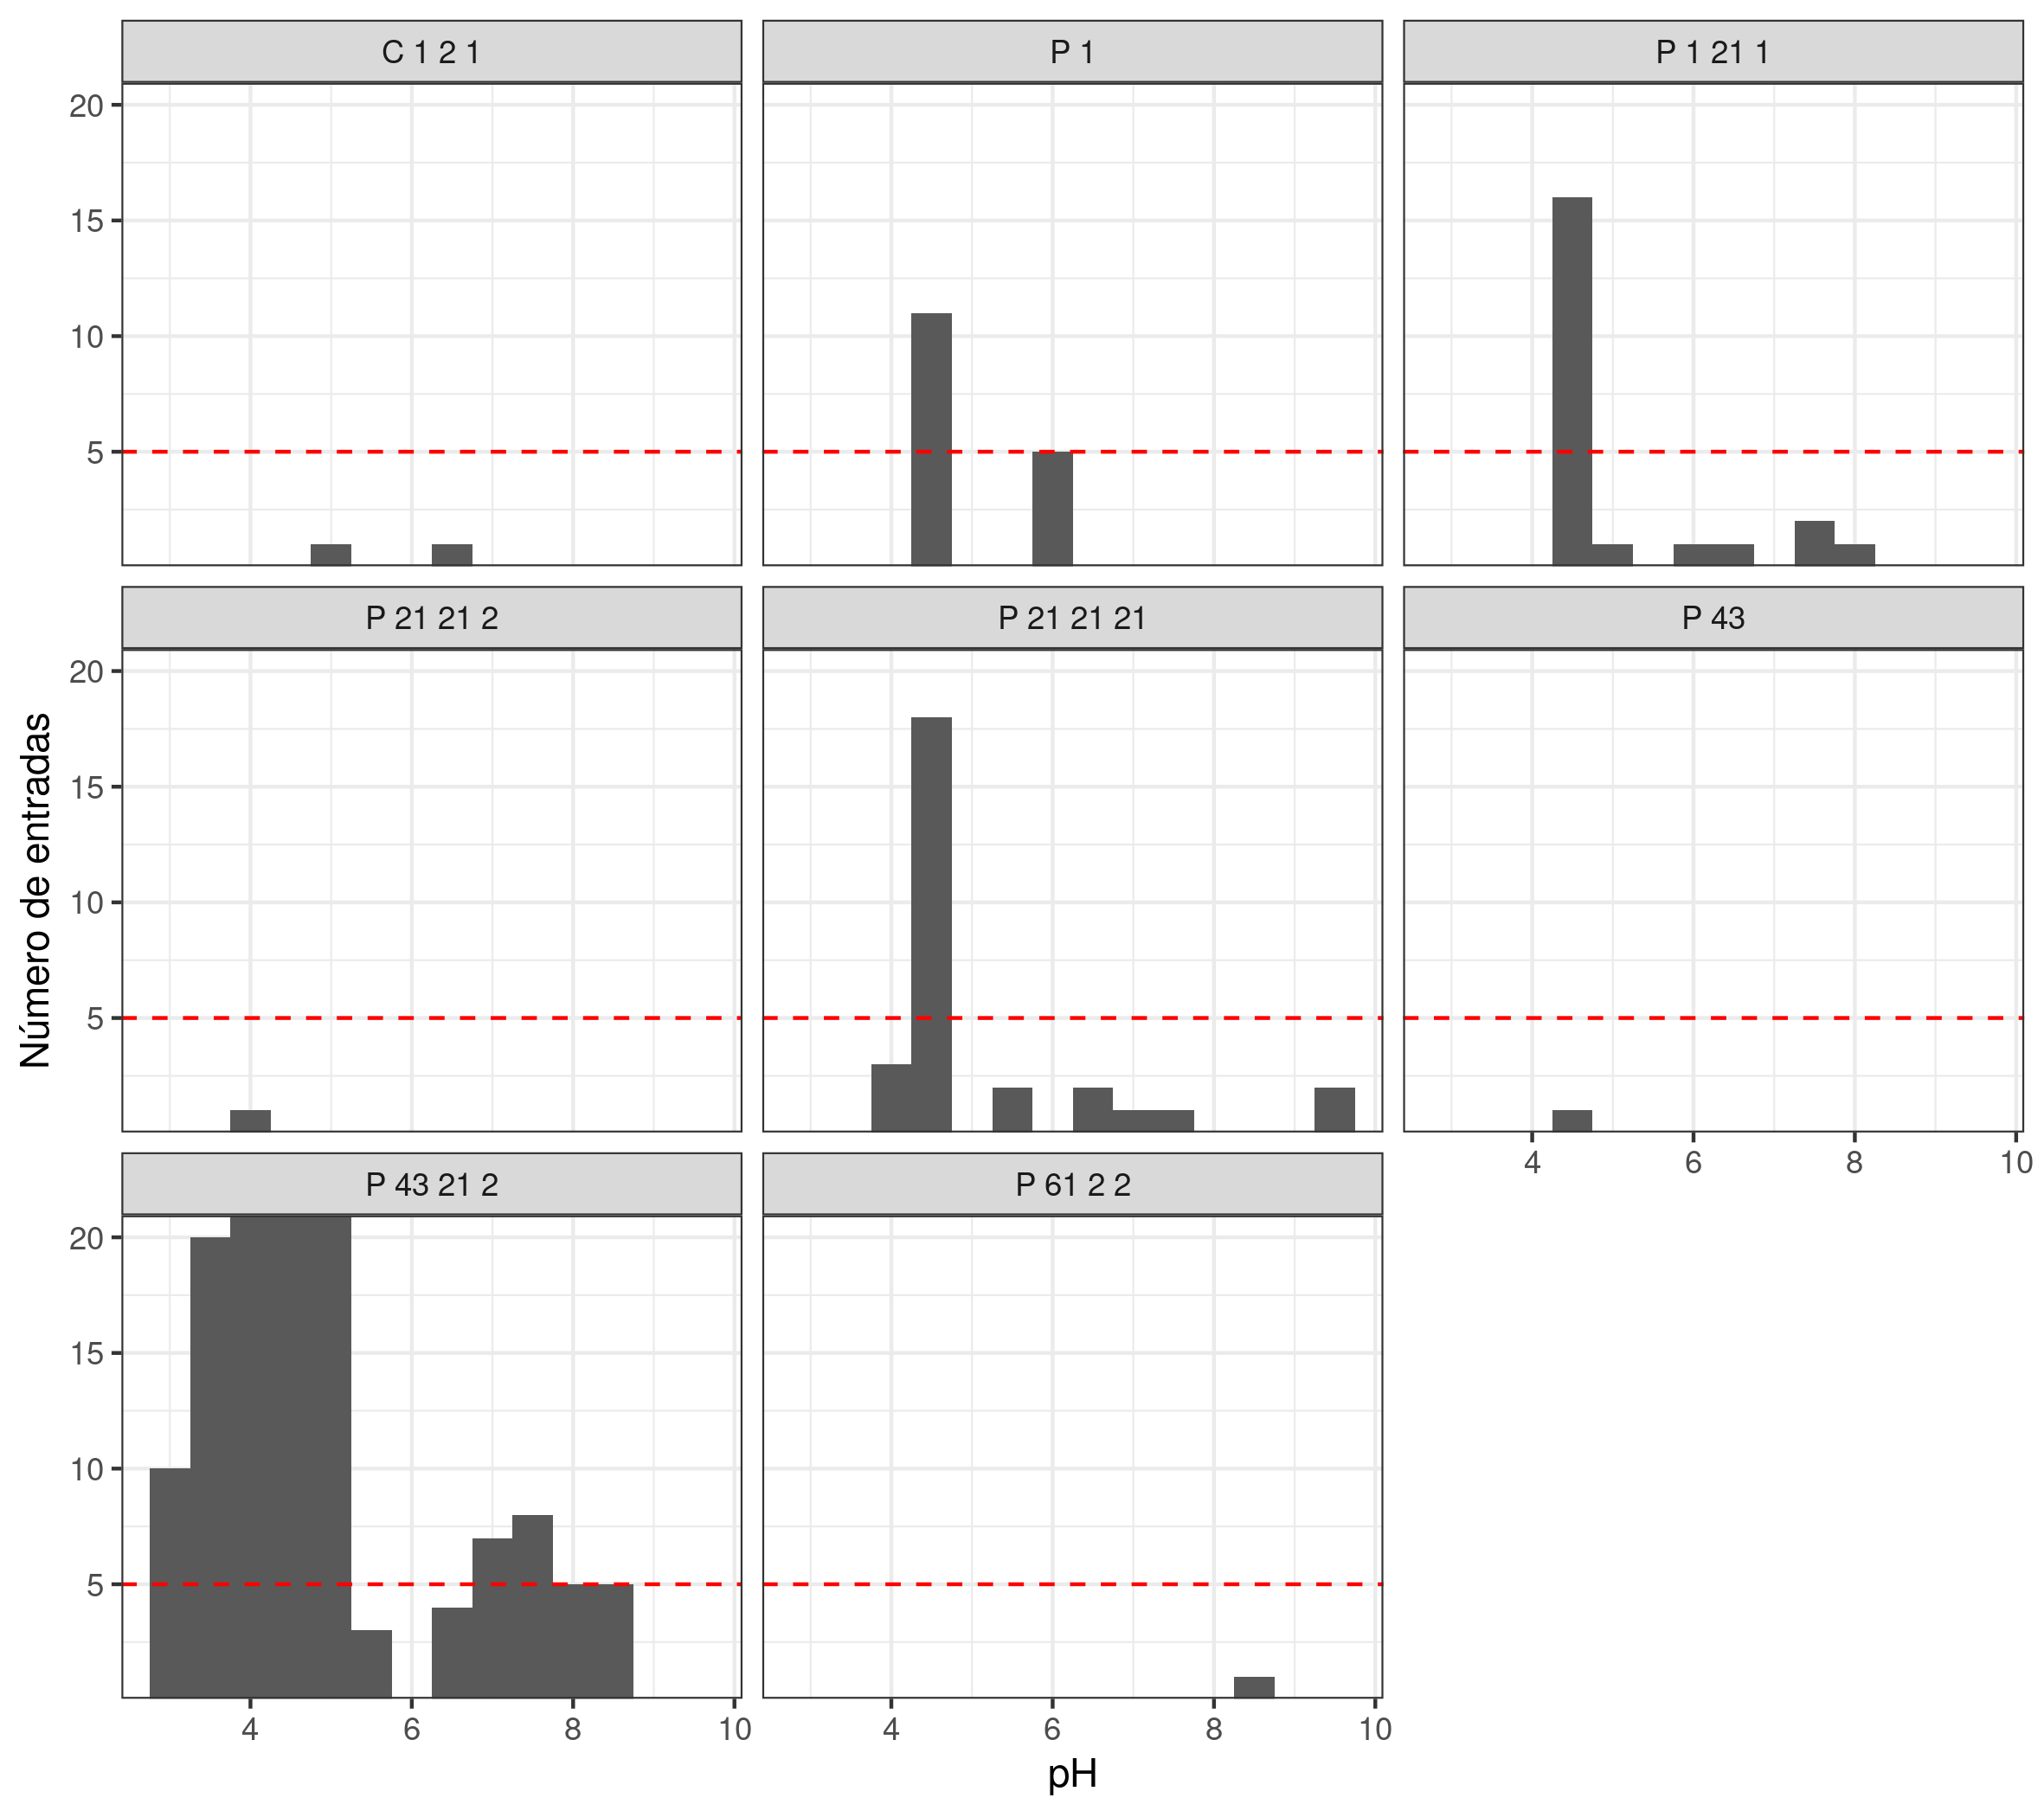
\includegraphics[width=0.8\textwidth]{imgs/hist_pH_by_gpo_P00698}
	\caption[Análisis visual]{Ejemplo del análisis visual: histograma de \texttt{P00698}. Nótese, en el gráfico de caja, que esta proteína tiene un amplio intervalo de pH $\sim~5$, en particular cuando cristaliza en el grupo espacial \texttt{P 43 21 2}. En este caso, la mayor parte de las estructuras están cristalizadas a un pH cercano a \num{4.7}, de ahí la forma final del gráfico de caja. Su frecuencia de cristalización en este mismo intervalo, según el histograma, es arriba de cinco (denotado por la línea horizontal roja), por lo  menos para buena parte del intervalo.}
	\labfig{fig:vis-anal}
\end{figure}
